\appendix

\chapter{Source Code}

The following code was used to manage, analyze, and graph output results from CH Instruments 1207 and 660B potentiostats that had been converted to text. It supports cyclic voltammetry, amperometry, and differential pulse voltammetry files. It is written for Python 2.5 and uses the Django package. Included here are only the files that perform management, analysis, and graphing. It is available in its entirety online at http://github.com/mjibson/biosensor/.

\singlespacing
\lstset{language=Python,basicstyle=\tiny,breaklines,tabsize=2}

biosensor/models.py:
\lstinputlisting{verbatim/biosensor/models.py}

biosensor/plot.awk:
\lstinputlisting{verbatim/biosensor/plot.awk}

biosensor/views.py:
\lstinputlisting{verbatim/biosensor/views.py}

\chapter{Screenshots}

The following screenshots are selected from the application described above.

\begin{figure}
	\centering
	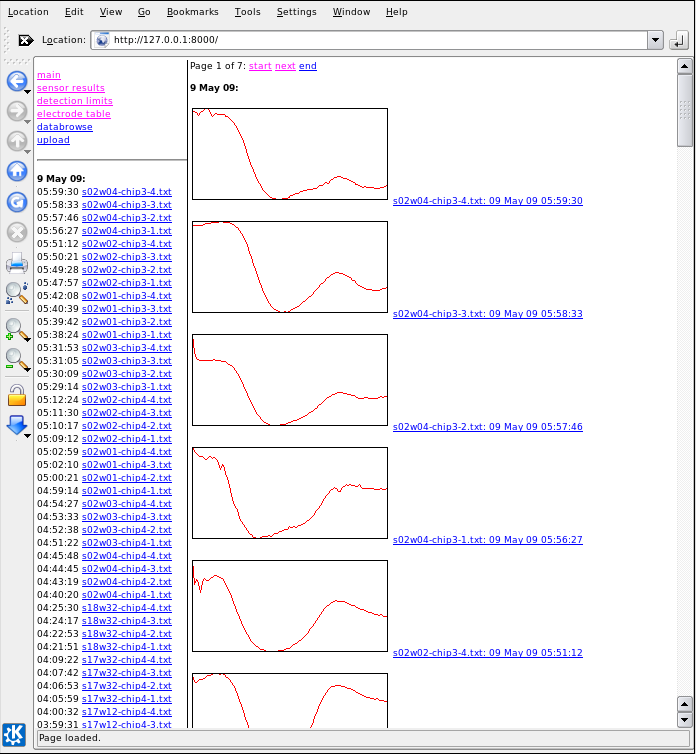
\includegraphics[width=\linewidth]{figures/web-main.png}
	\caption{Web application main page}
\end{figure}

\begin{figure}
	\centering
	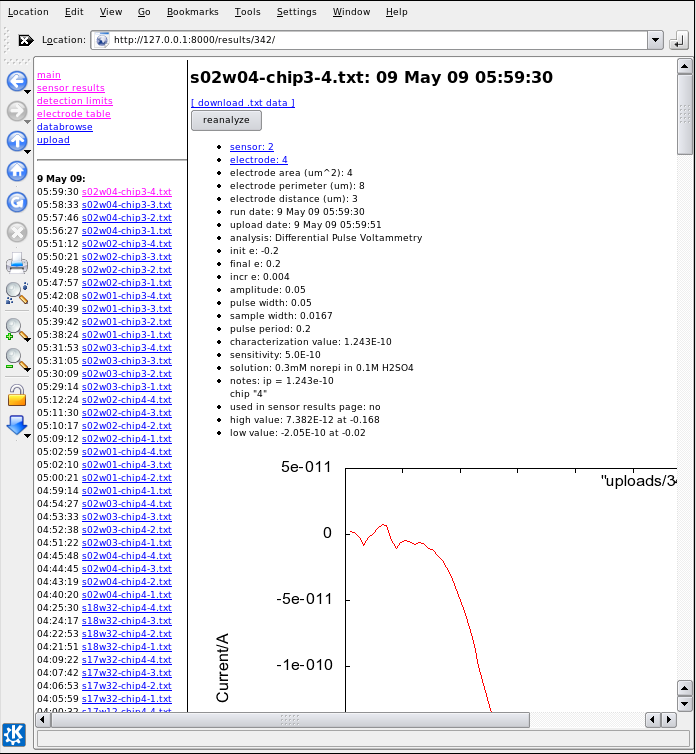
\includegraphics[width=\linewidth]{figures/web-detail.png}
	\caption{Web application result detail}
\end{figure}

\begin{figure}
	\centering
	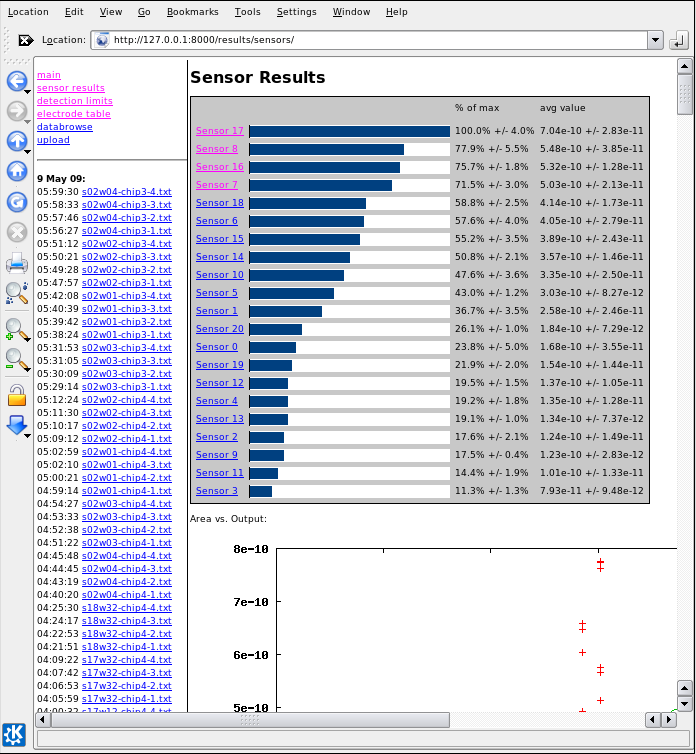
\includegraphics[width=\linewidth]{figures/web-sensors.png}
	\caption{Web application sensor results}
\end{figure}

\begin{figure}
	\centering
	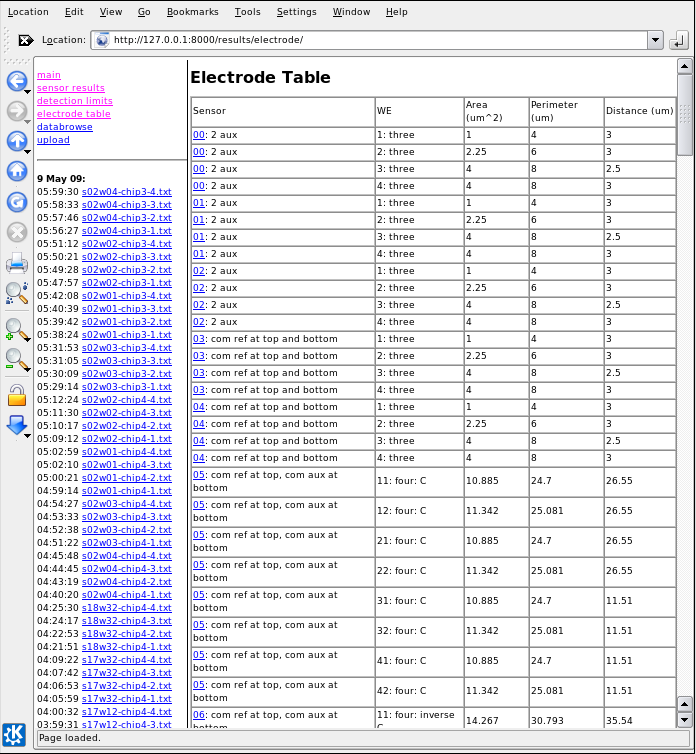
\includegraphics[width=\linewidth]{figures/web-electrodes.png}
	\caption{Web application electrode table}
\end{figure}
